\section{Lower Bounds}
Lower bounds are some of the most delightful things in computer science. In this case you analyse, not the complexity of a particular algorithm, but the complexity of a problem, in order to make statements about the minimum amount of effort required to solve a problem. In other words, you are finding what is the smallest runtime that \textit{any} algorithm solving the problem could have. 

Consider the example of sorting. We know we can sort in $O(n \log n)$ (via randomised quicksort for example). This gives an upper bound for the runtime of the best algorithm for sorting. If we knew the lower bound we could conclude that we had already found the best algorithm (up to asymptotic behaviour). But this is clearly a difficult problem: we would need to argue that \textit{every} algorithm solving the problem must run a certain amount of time. In practice, to make our lives easier we often classes or families of algorithms (i.e. algorithms that tackle the problem in similar ways). 

To continue the example with sorting, consider the class of algorithms that use pairwise comparison (i.e. the sorting is done by comparing pairs of elements in some manner). We can use comparison trees to represent such algorithms. 

\subsection{Comparison Trees}
In order to get used to arguing with comparison trees, let us consider the slightly different problem of searching through a sorted (1-based index) list and returning the index of the item if present. Suppose we are searching for an element in $x$ in a list $A$ where $A$ is of length 3. In the first step, we compare $x$ with $A[2]$ to determine whether $x$ should be on the first half of the list or the second half. Then we compare $x$ with $A[1]$ or $A[3]$ depending on the previous result (but not both). Now we know that $x$ is either at a specific index or not in the list at all. We can determine which of these it is with one final comparison. We can summarise all this in a comparison tree, see \autoref{fig:search-compar-tree}.

\begin{figure}[h]
    \centering
    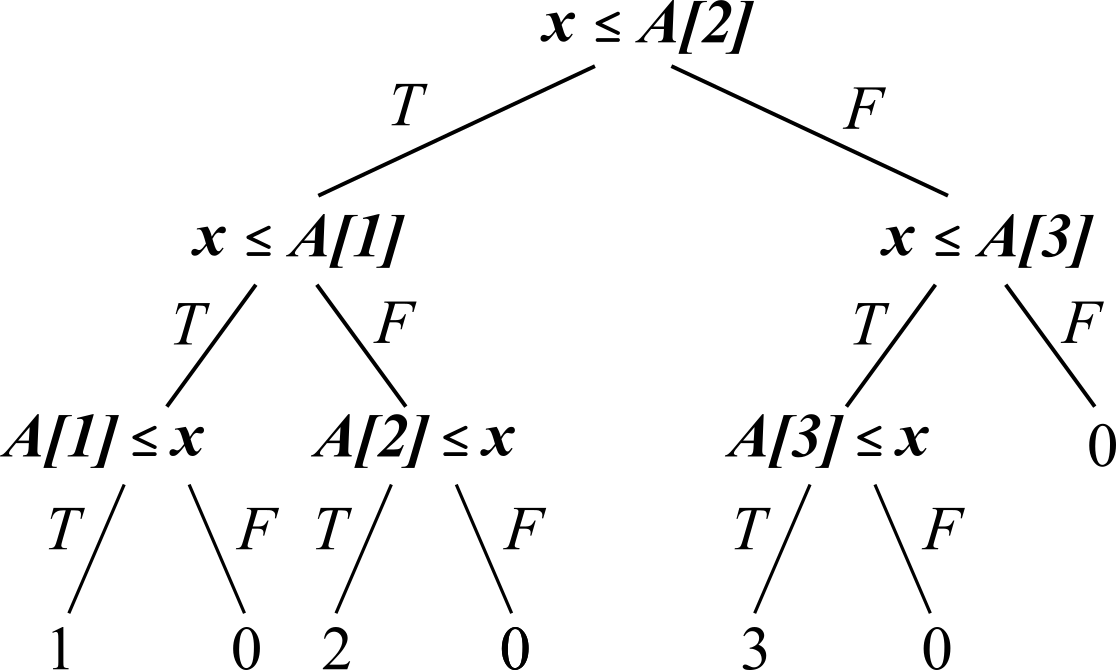
\includegraphics[scale=0.55]{Images/search_compar_tree.png}
    \caption{Comparison tree for binary search (return 0 if $x$ is not in the list)}
    \label{fig:search-compar-tree}
\end{figure}

Suppose a problem has $q$ possible outputs. This puts a lower bound on the height of the comparison tree since each output will correspond to at least one leaf. In particular, recall that a binary tree of height $h$ can have at most $2^h$ leaves. Conversely, if a binary tree is to have $q$ leaves then it must at least be of height $\lceil \log q \rceil$. The worst case runtime is proportional to the height of the tree and the expected runtime is proportional to the average depth of the leaves.
\begin{remark}
This means that searching in a sorted list with $q$ items is going to take at least $\Omega(\lceil \log (q + 1) \rceil) = \Omega(\log q)$ time. But binary search already has this runtime so we confirm that binary search is the fastest way of searching in a sorted list!
\end{remark}

\subsection{Sorting}
We now apply a similar analysis to the problem of sorting. First we make the problem precise: we seek an algorithm that will take as input a list of length $n$ and output a permutation of $[1, \dots, n]$ indicating the position (or rank as in \autoref{sec:aug-data-struc}) of each element. Thus for example, the output for $[2, 6, 3]$ would be $[1, 3, 2]$. The comparison tree for $n = 3$ might look like \autoref{fig:sorting-compar-tree}.

\begin{figure}[h]
    \centering
    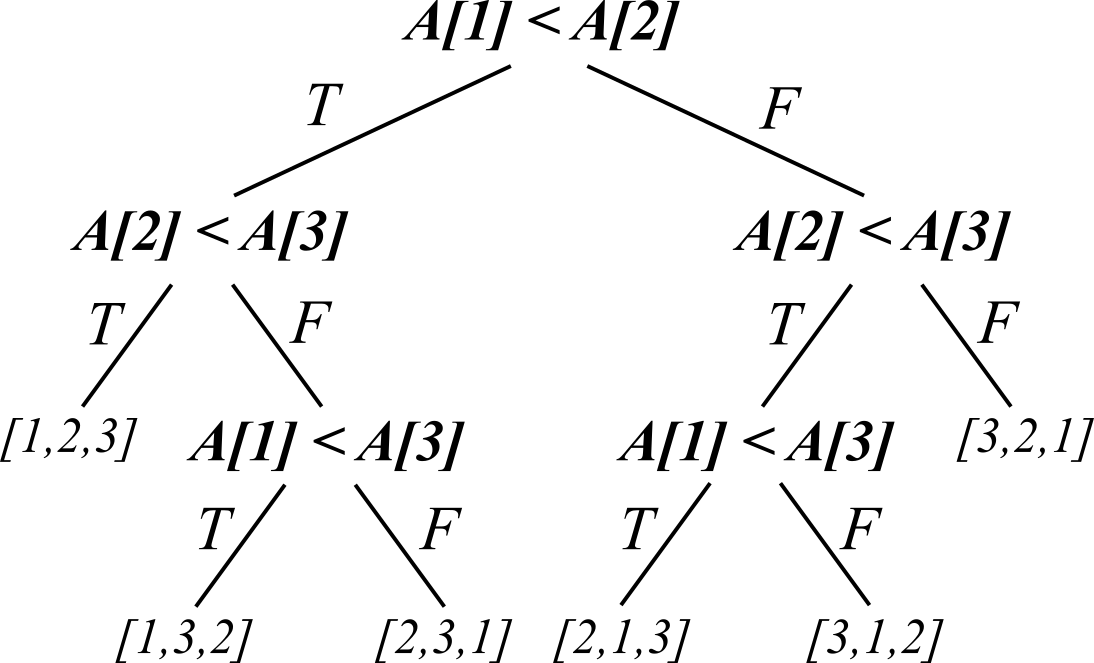
\includegraphics[scale=0.5]{Images/sorting_compar_tree.png}
    \caption{Comparison tree for sorting with $n = 3$}
    \label{fig:sorting-compar-tree}
\end{figure}

There are $n!$ possible outputs (the number of permutations of $[1, \dots, n]$) thus the height of comparison tree must be at $\log n!$. We claim that $\log n! = \Theta(n \log n)$ since
\begin{align*}
    \log n! &= \log n + \log(n - 1) + \dots + \log 2 + \log 1 \leq n \log n\\
    \log n! &= \log n + \log(n - 1) + \dots + \log 2 + \log 1 \geq \log n + \log(n - 1) + \dots + \log \frac{n}{2} \geq \frac{n}{2} \log \frac{n}{2}
\end{align*}
Thus any sorting algorithm that uses pairwise comparisons must take at least $\Theta(n \log n)$ time.

One does occasionally hear whispers of sorting being done in much faster time. How is this possible? The answer is cheating (kind of). We have found the lower bound for a very particular problem, if we change the problem slightly, for example by adding certain restrictions, we can get different lower bounds. A somewhat silly example is if we knew the elements of the list to be sorted were $n$ distinct elements from $[1, \dots, n]$. In this case, the algorithm could be made constant time by simply returning the input list. 
